\documentclass[10pt,pdf,hyperref={unicode}]{beamer}

\mode<presentation>
{
\usetheme{boxes}
\beamertemplatenavigationsymbolsempty

\setbeamertemplate{footline}[page number]
\usecolortheme{seagull}
\setbeamersize{text margin left=1.5em, text margin right=1.5em}
}

\usepackage[utf8]{inputenc}
\usepackage[english, russian]{babel}
\usepackage{bm}
\usepackage{multirow}
\usepackage{ragged2e}
\usepackage{indentfirst}
\usepackage{multicol}

\usepackage{graphicx}
\usepackage{caption}
\usepackage{subcaption}


\newtheorem{rustheorem}{Теорема}
\newtheorem{rusdefinition}{Определение}

\AtBeginEnvironment{figure}{\setcounter{subfigure}{0}}% Resets subfigure counter at start of figure environment

%----------------------------------------------------------------------------------------------------------
\title[\hbox to 56mm{Обучение с экспетом\hfill\insertframenumber\,/\,\inserttotalframenumber}]
{Задача обучения с экспертом для построения\\ интерпретируемых моделей машинного обучения}
\author[А.\,В.\;Грабовой]{\large Грабовой Андрей Валериевич}
\institute[]{Кафедра интеллектуального анализа данных\\Научный руководитель: д.ф.-м.н. В.\,В.\;Стрижов\\}

\date[2020]{Московский физико-технический институт\\8 декабря 2020 г.}
%----------------------------------------------------------------------------------------------------------

\begin{document}
%----------------------------------------------------------------------------------------------------------
\begin{frame}
\titlepage
\end{frame}

%----------------------------------------------------------------------------------------------------------
\begin{frame}{Обучение с экспертной информацией о данных}
\justifying
\textbf{Цель}

Предложить метод обучения выбора моделей машинного обучения на основе \textit{экспертной информацией} об исследуемых объектах.

~\\
\textbf{Исследуемая проблема}

Снижение размерности пространства параметров моделей глубокого обучения при помощи интерпретируемых моделей машинного обучения на основе экспертной информации.

~\\
\textbf{Требуется}

\begin{enumerate}
\justifying
	\item Формально поставить задача обучения на основе экспертного описания данных.
	\item Предложить метод решения на основе построения экспертного признакового описания объектов. 
	\item Использовать этот метод для решения задачи аппроксимации кривых второго порядка на бинарном изображении.
\end{enumerate}

\end{frame}

%----------------------------------------------------------------------------------------------------------
\begin{frame}{Список литературы}
\justifying
\begin{enumerate}
	\item \textit{Грабовой А.В., Стрижов В.В.} Анализ свойств вероятностных моделей обучения с экспертом~// в процессе подачи.
	\item \textit{Грабовой А.В., Стрижов В.В.} Анализ выбора априорного распределения для смеси экспертов // Журнал Вычислительной математики и математической физики, 2021. Т.\,61. \textnumero\,5.
	\item \textit{Yuksel Seniha Esen, Wilson Joseph N., Gader Paul D} Twenty Years of Mixture of Experts~// IEEE Transactions on Neural Networks and Learning Systems, 2012. Vol.\,23. No\,8. Pp.\,1177--1193.
\end{enumerate}
\end{frame}

%----------------------------------------------------------------------------------------------------------

\begin{frame}{Аппроксимации кривых второго порядка}
\justifying
\begin{center}
	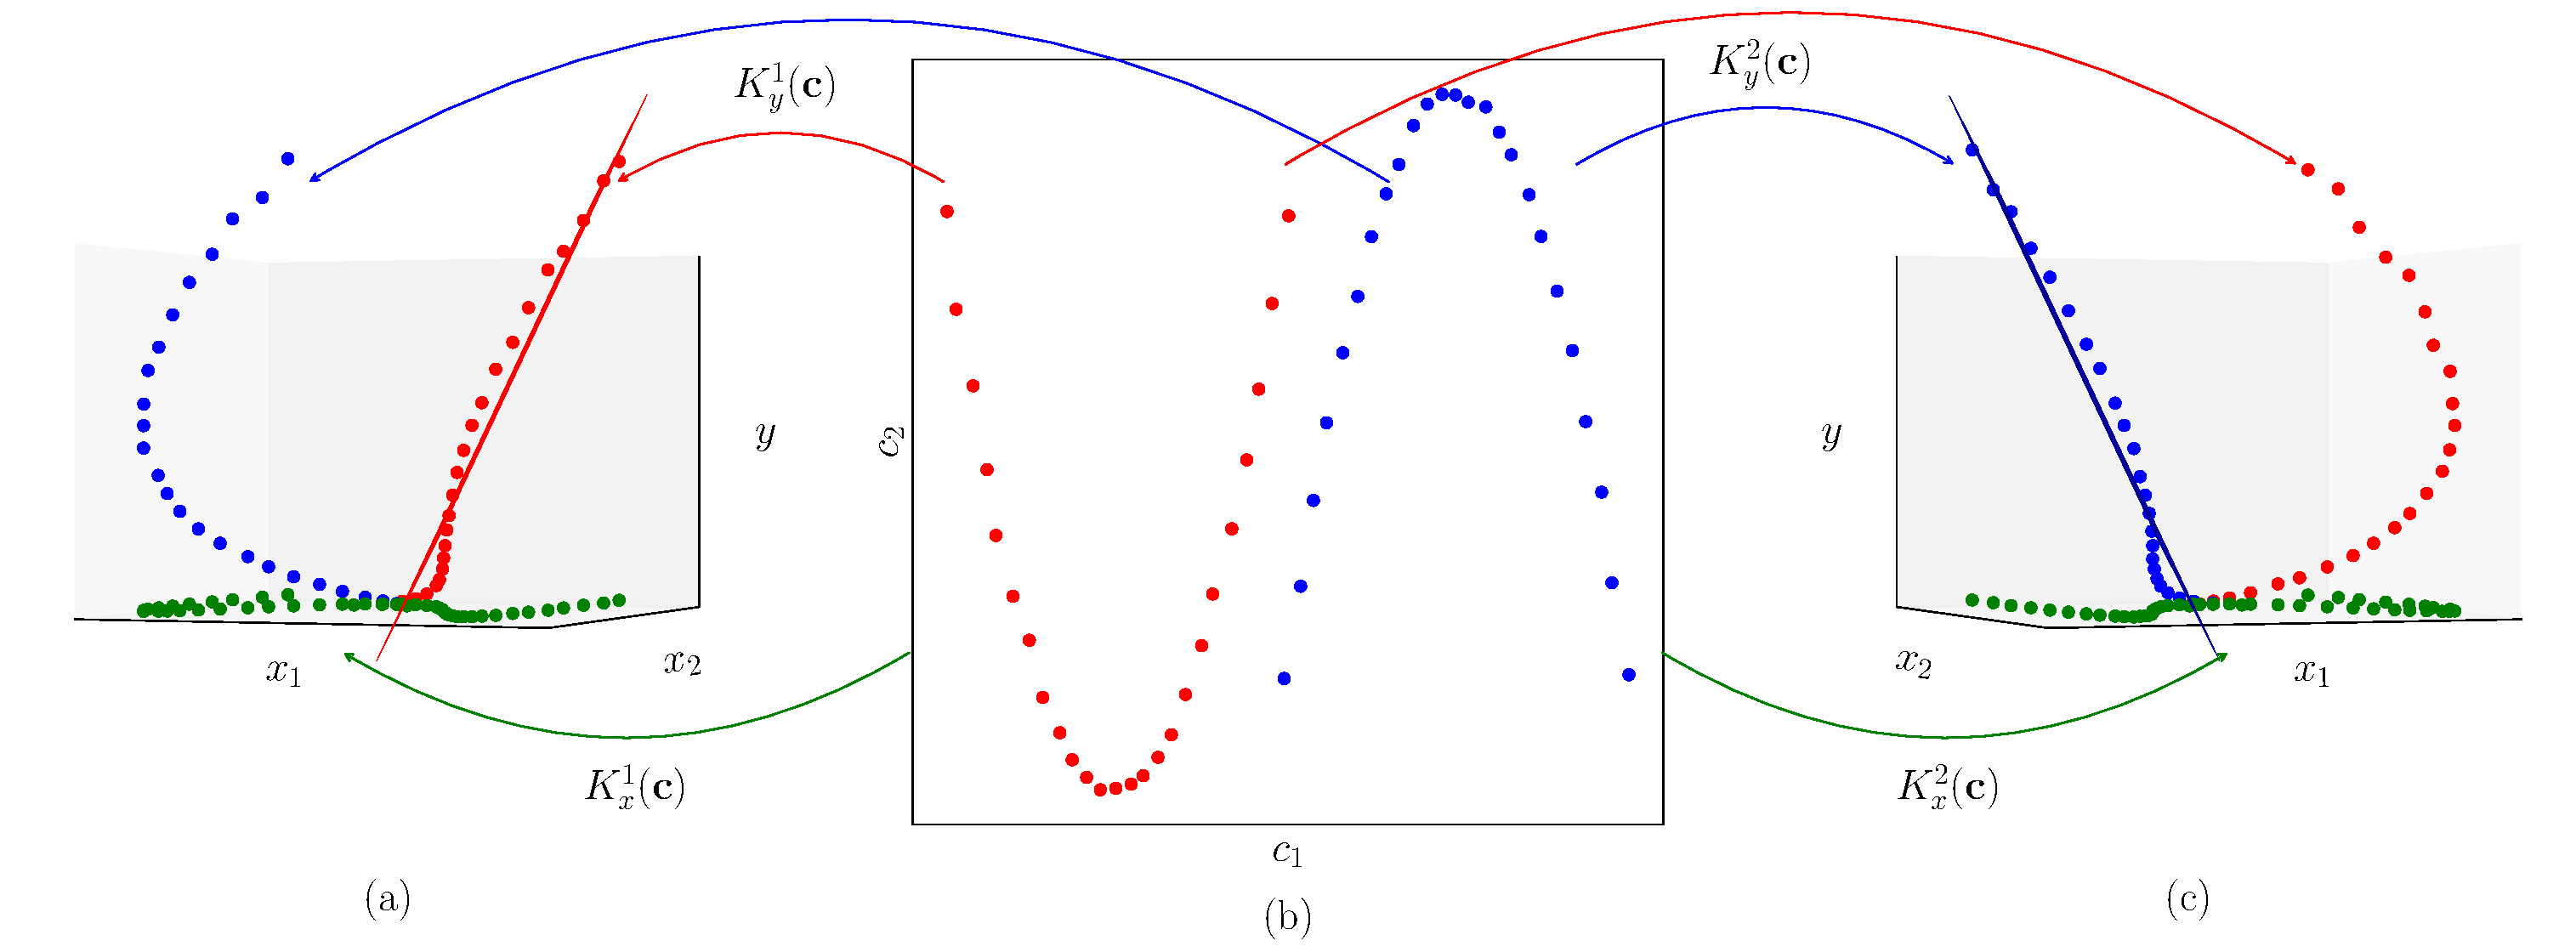
\includegraphics[width=0.9\textwidth]{figures/explanation}
\end{center}

\begin{enumerate}
    \item[(b)] Исходный набор точек на изображении.
    \item[(a)] Представление первого эксперта: $K^{1}_x, K^{1}_y$ --- отображение в данное представление.
    \item[(c)] Представление второго эксперта: $K^{2}_x, K^{2}_y$ --- отображение в данное представление.
\end{enumerate}

\end{frame}

%----------------------------------------------------------------------------------------------------------

\begin{frame}{Постановка задачи: кривые второго порядка}
\justifying
Изображение
\[
\mathbf{M} \in \{0,1\}^{m_1\times m_2},
\]
где $1$~--- точка изображение,  а $0$~--- точка фона. 

Точки изображения --- кривая второго порядка~$\Omega$.
Координаты точек изображения $\mathbf{C} \in \mathbb{R}^{N\times2}$.
Задана экспертная информация $E\bigr(\Omega\bigr)$ о фигуре~$\Omega$.

Признаковое описание экспертов:
\[
K_x\bigr(E\bigr(\Omega\bigr)\bigr):\mathbb{R}^{2} \to \mathbb{R}^{n},
\quad K_y\bigr(E\bigr(\Omega\bigr)\bigr): \mathbb{R}^{2} \to \mathbb{R},
\]
где $K_x, K_y$ отображения в признаковое описание и пространство ответов.

Набор данных для аппроксимации кривых:
\[
\mathfrak{D} = \{(\mathbf{x}, y) \; | \; \forall \mathbf{c} \in \mathbf{C} \;\quad \mathbf{x} = K_x(\mathbf{c}), \; y = K_y(\mathbf{c}) \}.
\]

В данной работе предполагается, что выборка~$\mathfrak{D}$ аппроксимируется линейной моделью
$
	g(\mathbf{x}, \mathbf{w}) = \mathbf{x}^\mathsf{T} \mathbf{w},
$
где~$\mathbf{w}$ вектор, параметр, который требуется найти.


Требуется решить оптимизационную задачу:
\[
	\hat{\mathbf{w}} = \arg\min_{\mathbf{w}\in\mathbb{R}^n} \sum_{\left(\mathbf{x}, y\right) \in \mathfrak{D}}\|g(\mathbf{x}, \mathbf{w}) - y \|_2^2.
\]
\end{frame}

%----------------------------------------------------------------------------------------------------------

\begin{frame}{Постановка задачи: признаковое описание кривых}
\justifying
Кривая второго порядка: главная ось которой не параллельна оси ординат:
\[
\setlength\abovedisplayskip{0pt}
x^2 = B'xy+C'y^2+D'x+E'y+F',
\setlength\belowdisplayskip{0pt}
\]
также на коэффициенты $B',C'$ могут быть наложены ограничения. 

Отображение в экспертное описание:
\[
\setlength\abovedisplayskip{0pt}
K_x\bigr(\mathbf{c}_i\bigr)=\left[x_iy_i, y_i^2, x_i, y_i, 1\right], \quad K_y\bigr(\mathbf{c}_i\bigr)=x_i^2.
\setlength\belowdisplayskip{0pt}
\]

\begin{columns}
\column{0.64\textwidth}
\textbf{Частный случай: аппроксимации окружности}

Пусть $x_0, y_0$~--- центр окружности, которую требуется найти, а $r$ ее радиус.

Точки~$\left(x_i, y_i\right)\in\textbf{C}$ удовлетворяют уравнению окружности:
\[
\setlength\abovedisplayskip{0pt}
\begin{aligned}
\left(x_i - x_0\right)^{2}+\left(y_i-y_0\right)^2 = r^2 \Rightarrow\\
\Rightarrow(2x_0)\cdot x_i + (2y_0)\cdot y_i+(r^2-x_0^2-y_0^2)\cdot1 = x_{i}^2 + y_{i}^2.
\end{aligned}
\setlength\belowdisplayskip{0pt}
\]
\column{0.36\textwidth}
\begin{center}
	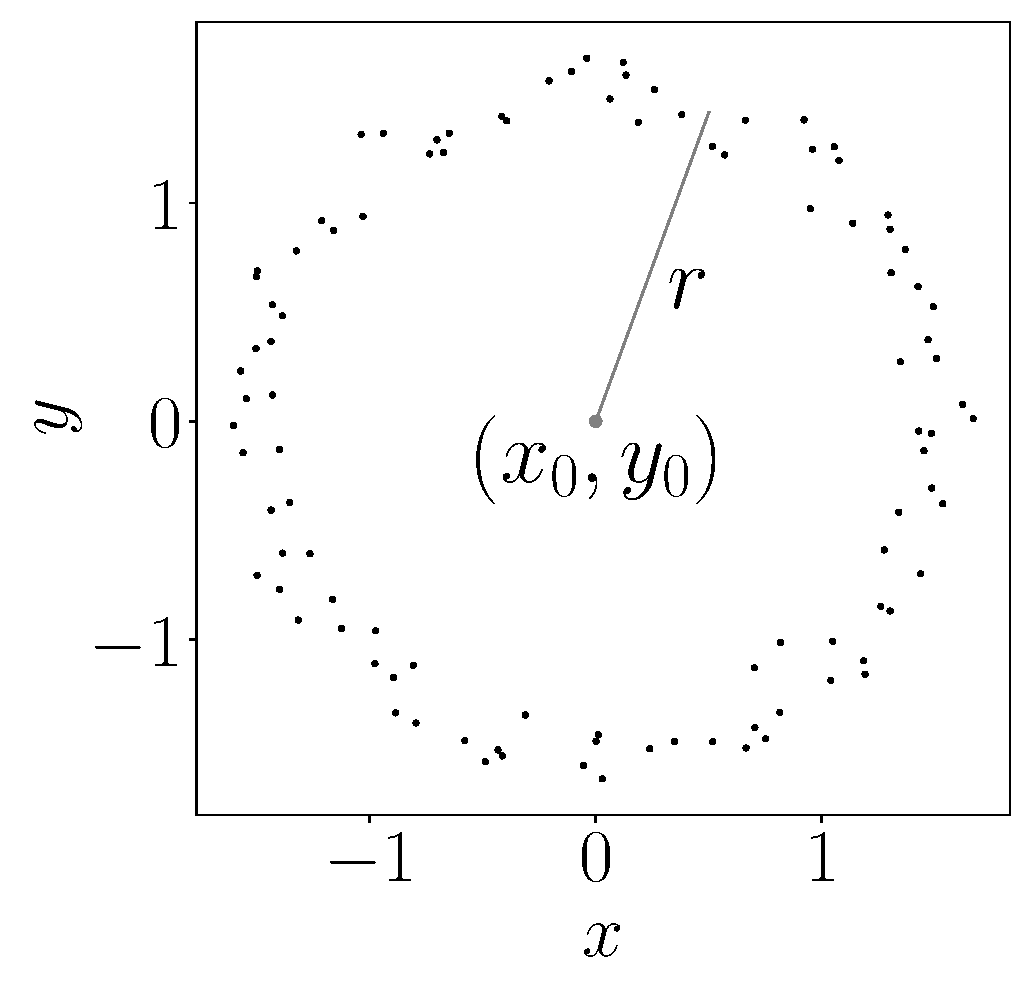
\includegraphics[height=0.37\textheight]{figures/slides_statment}
\end{center}
\end{columns}

Линейная регрессия для аппроксимации окружности:
\[
\setlength\abovedisplayskip{0pt}
\begin{aligned}
\textbf{X}\textbf{w} \approx \textbf{y},  \quad \textbf{X} = \left[\textbf{C}, \textbf{1}\right], \quad \textbf{y} = [x_1^2+y_1^2, x_2^2+y_2^2, \cdots, x_N^2+y_N^2]^{\mathsf{T}},
\end{aligned}
\setlength\belowdisplayskip{0pt}
\]
где оптимальные параметры $\textbf{w} = \bigr[w_1, w_2, w_3\bigr]^{\mathsf{T}}$ восстанавливают окружность:
\[
\setlength\abovedisplayskip{0pt}
\begin{aligned}
x_0 = \frac{w_1}{2}, \quad y_0 = \frac{w_2}{2}, \quad r = \sqrt[]{w_3+x_{0}^{2}+y_{0}^{2}}.
\end{aligned}
\setlength\belowdisplayskip{0pt}
\]


\end{frame}

%----------------------------------------------------------------------------------------------------------

\begin{frame}{Постановка задачи: мультимодель}
\justifying
Заданы $K$ кривых второго порядка $\Omega_1, \cdots, \Omega_K$ с $E_k = E\bigr(\Omega_k\bigr)$.

\begin{rusdefinition}
Функция $f$ называется смесью K экспертов, если:
\[
	f = \sum\limits_{k = 1}^{K}\pi_k(\mathbf{x}, \mathbf{V})g_k(\mathbf{w}_k),  \quad \pi_k(\mathbf{x}, \mathbf{V}): \mathbb{R}^{n\times |\mathbf{V}|} \rightarrow [0, \, 1], \quad \sum\limits_{k = 1}^{K}\pi_k(\mathbf{x}, \mathbf{V}) = 1, 
\]
где $g_k$~---~локальная модель, $\mathbf{x}$~---~признаки, $\pi_k$~---~шлюзовая функция, $\mathbf{w}_k$~---~параметры, $\mathbf{V}$~---~параметры шлюзовой функции.
\end{rusdefinition}

Мультимодель, описывающую кривые $\Omega_1, \dots, \Omega_K$ на изображении $\mathbf{M}$:
\[
\setlength\abovedisplayskip{0pt}
	f = \sum_{k = 1}^{K} \pi_k(\mathbf{c}, \mathbf{V})g_k(K^k_{x}\bigl(\mathbf{c}), \mathbf{w}_k), \quad \mathbf{x}=K^1_{x}\bigl(\mathbf{c})=\cdots=K^K_{x}\bigl(\mathbf{c}).
\setlength\belowdisplayskip{0pt}
\]
Требуется решить оптимизационную задачу:
\[
\setlength\abovedisplayskip{0pt}
\mathcal{L} = \sum\limits_{(\mathbf{x}, y) \in \mathfrak{D}} \sum\limits_{k = 1}^{K} \pi_k(\mathbf{x}, \mathbf{V})(y - \mathbf{w}_k^{\mathsf{T}}\mathbf{x})^2 + R\bigl(\mathbf{V}, \mathbf{W}, E(\Omega)\bigr) \rightarrow \min_{\mathbf{V}, \mathbf{W}},
\setlength\belowdisplayskip{0pt}
\]
где $\mathbf{W} = [\mathbf{w}_1, \dots, \mathbf{w}_k]$~--- параметры локальных моделей, $R\bigl(\mathbf{V}, \mathbf{W}, E(\Omega)\bigr)$~---~регуляризация параметров, основанная на экспертной информации.

\end{frame}

%----------------------------------------------------------------------------------------------------------

\begin{frame}{Вероятностная постановка задачи}
\justifying

Заданы:
\begin{enumerate}
	\item[1)] правдоподобие выборки $p_{k}\left(y_{i}|\mathbf{w}_{k}, \mathbf{x}_{i}\right) = \mathcal{N}\left(y_{i}|\mathbf{w}_{k}^{\mathsf{T}}\mathbf{x}_{i}, \beta^{-1}\right),$ где $\beta$ уровень шума,
	\item[2)] априорное распределение параметров $p^{k}\left(\mathbf{w}_{k}\right) = \mathcal{N}\left(\mathbf{w}_{k}|\mathbf{w}^{0}_{k}, \mathbf{A}_{k}\right),$ где $\mathbf{w}^{0}_{k}$~---~вектор размера $n\times1,$ $\mathbf{A}_{k}$~---~ковариационная матрица параметров,
	\item[3)] регуляризация априорного распределения $p\left(\bm{\varepsilon}_{k,k'}|\bm{\alpha}\right) = \mathcal{N}\left(\bm{\varepsilon}_{k,k'}|\mathbf{0},  \bm{\Xi}\right),$ где~$\bm{\Xi}$~---~ковариационная матрица общего вида, $\bm{\varepsilon}_{k,k'} = \mathbf{w}_{k}^{0}-\mathbf{w}_{k'}^{0}.$
\end{enumerate}

Правдоподобие модели включает правдоподобие выборки, априорное распределение параметров, а также их регуляризацию
\[
\begin{aligned}
p\bigr(\mathbf{y}, \mathbf{W}|\mathbf{X}, \mathbf{V}, \textbf{A}, \textbf{W}^{0}, \bm{\Xi}, \beta\bigr) = &\prod_{k,k'=1}^{K}\mathcal{N}\left(\bm{\varepsilon}_{k,k'}|\mathbf{0},  \bm{\Xi}\right)\cdot\\
&\cdot\prod_{k=1}^{K}\mathcal{N}\left(\mathbf{w}_{k}|\mathbf{w}^{0}_{k}, \mathbf{A}_{k}\right)\prod_{i=1}^{N}\left(\sum_{k=1}^{K}\pi_{k}\mathcal{N}\left(y_{i}|\mathbf{w}_{k}^{\mathsf{T}}\mathbf{x}_{i}, \beta^{-1}\right)\right),
\end{aligned}
\]
где~$\mathbf{A} = \bigr\{\mathbf{A}_1, \cdots, \mathbf{A}_K\bigr\}.$

\end{frame}

%----------------------------------------------------------------------------------------------------------

\begin{frame}{Оптимизационная задача}
\justifying

Введем скрытые переменные $\textbf{Z} = [z_{ik}],$ где $~z_{ik} = 1$ тогда и только тогда, когда $k_i=k$:
\[
\begin{aligned}
\log p\bigr(\mathbf{y}, &\mathbf{Z}, \mathbf{W}|\mathbf{X}, \mathbf{V}, \textbf{A}, \textbf{W}^{0},  \bm{\Xi}, \beta\bigr) =\\
&= \sum_{i=1}^{N}\sum_{k=1}^{K}z_{ik}\left[\log\pi_k\left(\textbf{x}_i, \textbf{V}\right) - \frac{\beta}{2}\left(y_{i} - \textbf{w}_{k}^{\mathsf{T}}\textbf{x}_{i}\right)^{2} + \frac{1}{2}\log\frac{\beta}{2\pi}\right] +\\
&+ \sum_{k=1}^{K}\left[-\frac{1}{2}\left(\textbf{w}_{k} - \textbf{w}_{k}^{0}\right)^{\mathsf{T}}\textbf{A}_{k}^{-1}\left(\textbf{w}_{k} - \textbf{w}_{k}^{0}\right) + \frac{1}{2}\log\det\textbf{A}^{-1}_{k} - \frac{n}{2}\log2\pi\right]+\\
&+ \sum_{k=1}^{K}\sum_{k'=1}^{K}\left[-\frac{1}{2}\left(\textbf{w}_{k}^{0}-\textbf{w}_{k'}^{0}\right)^{\mathsf{T}}\hat{\bm{\alpha}}^{-1}\left(\textbf{w}_{k}^{0}-\textbf{w}_{k'}^{0}\right) +\frac{1}{2}\log\det \bm{\Xi} -\frac{n}{2}\log{2\pi}\right].
\end{aligned}
\]

Задача оптимизации параметров локальных моделей и параметров смеси принимает следующий вид:
\[
\begin{aligned}
\mathbf{W}, \mathbf{Z}, \mathbf{V}, \mathbf{W}^0, \textbf{A},  \beta = \arg\max_{\mathbf{W}, \mathbf{Z}, \mathbf{V}, \mathbf{W}^0, \textbf{A}, \beta} \log p\bigr(\mathbf{y}, \mathbf{Z}, \mathbf{W}&|\mathbf{X}, \mathbf{V}, \textbf{A}, \textbf{W}^{0}, \bm{\Xi}, \beta\bigr).
\end{aligned}
\]

Для оптимизации используется вариационный ЕМ--алгоритм с предположением~$q\left(\textbf{Z}, \textbf{W}\right) = q\left(\textbf{Z}\right)q\left(\textbf{W}\right)$.
\end{frame}

%----------------------------------------------------------------------------------------------------------
\begin{frame}{EM--алгоритм для решения задачи смеси экспертов}
\justifying
Итерационные формулы ЕМ--алгоритма:
	\begin{enumerate}
		\item Е--шаг: 
			\begin{equation*}
				\begin{aligned}
					&p\left(z_{ik} = 1\right) = \frac{\exp\left(\log\pi_{k}\left(\textbf{x}_{i}, \textbf{V}\right) - \frac{\beta}{2}\left(\textbf{x}_{i}^{\mathsf{T}}\mathsf{E}\textbf{w}_{k}\textbf{w}_{k}^{\mathsf{T}}\textbf{x}_{i} - \textbf{x}_{i}^{\mathsf{T}}\mathsf{E}\textbf{w}_{k}\right)\right)}{\sum_{k'=1}^{K}\exp\left(\log\pi_{k'}\left(\textbf{x}_{i}, \textbf{V}\right) - \frac{\beta}{2}\left(\textbf{x}_{i}^{\mathsf{T}}\mathsf{E}\textbf{w}_{k'}\textbf{w}_{k'}^{\mathsf{T}}\textbf{x}_{i} - \textbf{x}_{i}^{\mathsf{T}}\mathsf{E}\textbf{w}_{k'}\right) \right)},\\
					&q(\textbf{w}_k) = \mathcal{N}(\textbf{w}_k|\textbf{m}_k, \textbf{B}_k),\\
					&\mathbf{m}_{k} = \mathbf{B}_{k}\left(\mathbf{A}_{k}^{-1}\mathbf{w}_{k}^{0}+\beta\sum_{i=1}^{N}\mathbf{x}_{i}y_{i}\mathsf{E}z_{ik}\right), \quad
					\mathbf{B}_{k} = \left(\mathbf{A}_{k}^{-1}+\beta\sum_{i=1}^{N}\mathbf{x}_{i}\mathbf{x}_{i}^{\mathsf{T}}\mathsf{E}z_{ik}\right)^{-1} .
				\end{aligned}
			\end{equation*}
		\item М--шаг: 
			\begin{equation*}
				\begin{aligned}
					&\textbf{A}_{k} = \mathsf{E}\textbf{w}_{k}\textbf{w}_{k}^{\mathsf{T}} - \textbf{w}_{k}^{0}\mathsf{E}\textbf{w}_{k}^{\mathsf{T}} - \mathsf{E}\textbf{w}_{k}\textbf{w}_{k}^{0\mathsf{T}} + \textbf{w}_{k}^{0}\textbf{w}_{k}^{0\mathsf{T}}, \\
					 &\frac{1}{\beta}=\frac{1}{N}\sum_{i=1}^{N}\sum_{k=1}^{K}\left[y_{i}^{2}-2y_{i}\textbf{x}_{i}^{\mathsf{T}}\mathsf{E}\textbf{w}_{k} + \textbf{x}_{i}^{\mathsf{T}}\mathsf{E}\textbf{w}_{k}\textbf{w}_{k}^{\mathsf{T}}\textbf{x}_{i}\right]\mathsf{E}z_{ik},\\
					&\textbf{w}_{k}^{0} =\left[\textbf{A}_{k}^{-1}+\left(K-1\right)\bm{\Xi}\right]^{-1}\left(\textbf{A}^{-1}_{k}\mathsf{E}\textbf{w}_{k}+\bm{\Xi}\sum_{k'=1,~k'\not=k}^{K}\textbf{w}_{k'}^{0}\right),\\
					&\textbf{V}= \arg\max_{\textbf{V}} \mathsf{E}_{q^{s}}\log p\bigr(\mathbf{y}, \textbf{Z},\mathbf{W}|\mathbf{X}, \mathbf{V}, \textbf{A}, \textbf{W}^{0}, \bm{\Xi}, \beta\bigr).
				\end{aligned}
			\end{equation*}
	\end{enumerate}
\end{frame}
%----------------------------------------------------------------------------------------------------------


\begin{frame}{Вычислительный эксперимент}
\justifying
\textbf{Эксперимент с окружностями:}
\begin{enumerate}
\item Синтетическое изображение трех непересекающих окружностей с шумом.
\item Сравнивается модели: с заданием априорного распределения и без него.
\end{enumerate}

\textbf{Эксперимент с разным уровнем шума в данных:}

\begin{enumerate}
\item Синтетическое изображение двух парабол.
\item Анализ качества аппроксимации~$S$ от уровня шума~$\beta$ в данных и от параметра априорных распределений~$\gamma$. Качество аппроксимации следующее:
\[
\setlength\abovedisplayskip{0pt}
S = ||\mathbf{w}^\text{pred}_{1} - \mathbf{w}^\text{true}_{1}||^{2}_{2} + ||\mathbf{w}^\text{pred}_{2} - \mathbf{w}^\text{true}_{2}||^{2}_{2}.
\setlength\belowdisplayskip{0pt}
\]
\end{enumerate}

\textbf{Аппроксимация радужки глаза}
\begin{enumerate}
	\item Реальные изображения радужки глаза с предобработкой для их бинаризации. 
	\item Сравниваются различные регуляризаторы:
	\begin{itemize}
		\item $R_0\bigl(\mathbf{V}, \mathbf{W}, E(\Omega)\bigr)=0$;
		\item $R_1\bigl(\mathbf{V}, \mathbf{W}, E(\Omega)\bigr)= -\sum_{k=1}^{K}\mathbf{w}_k^{\mathsf{T}}\mathbf{w}_k$;
		\item $R_2\bigl(\mathbf{V}, \mathbf{W}, E(\Omega)\bigr)= -\sum_{k=1}^{K}\mathbf{w}_k^{\mathsf{T}}\mathbf{w}_k + \sum_{k=1}^{K}\sum_{k'=1}^{K}\sum_{j=1}^2\left(w_k^j-w_{k'}^j\right)^2$.
	\end{itemize}
\end{enumerate}


\end{frame}
%----------------------------------------------------------------------------------------------------------

\begin{frame}{Эксперимент с окружностями}
\justifying

\begin{figure}[h!]
\begin{minipage}{.25\textwidth}
      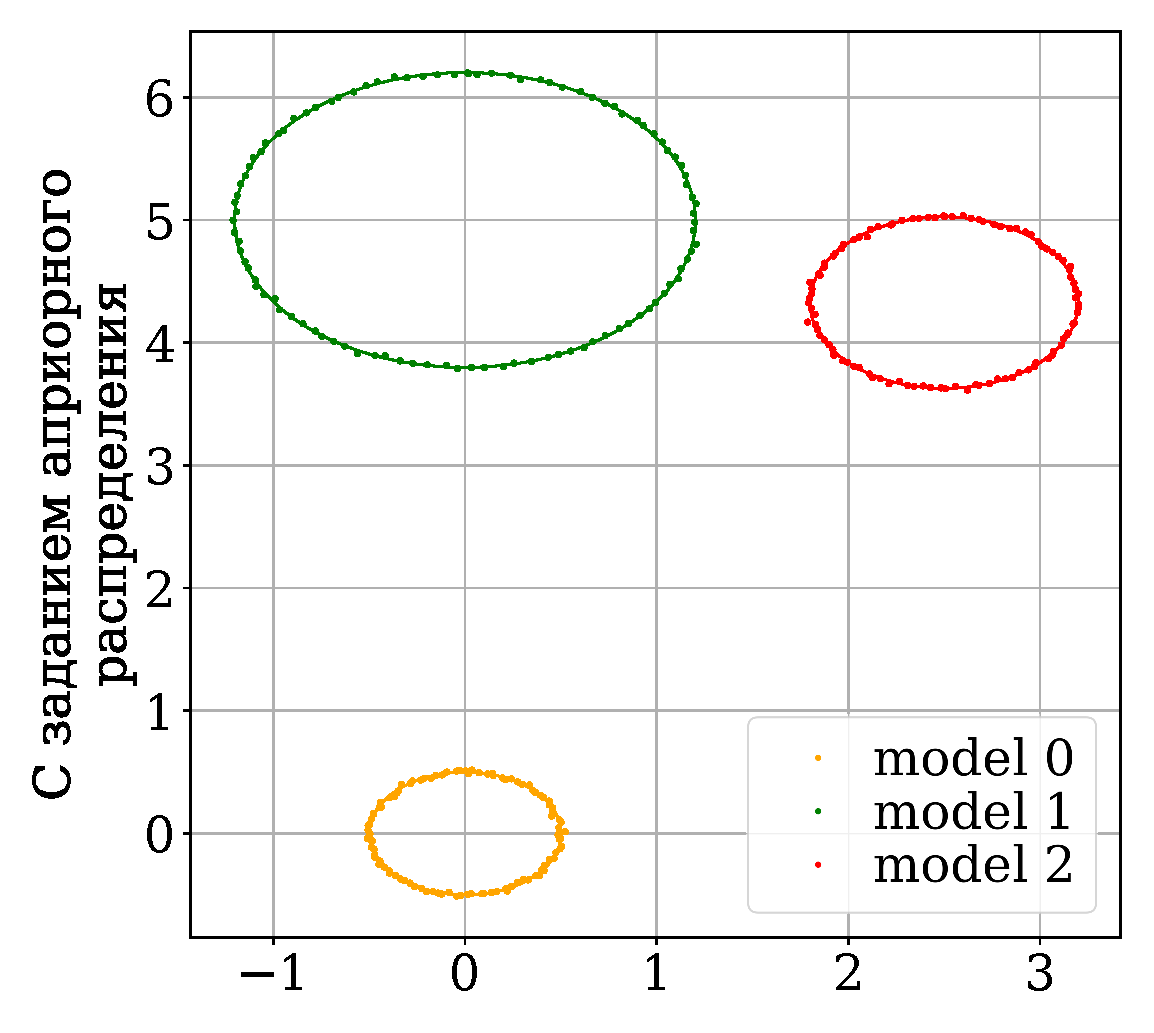
\includegraphics[width =  1.0\textwidth]{figures/910.eps}
\end{minipage}
\begin{minipage}{.25\textwidth}
\hspace{0.3mm}
      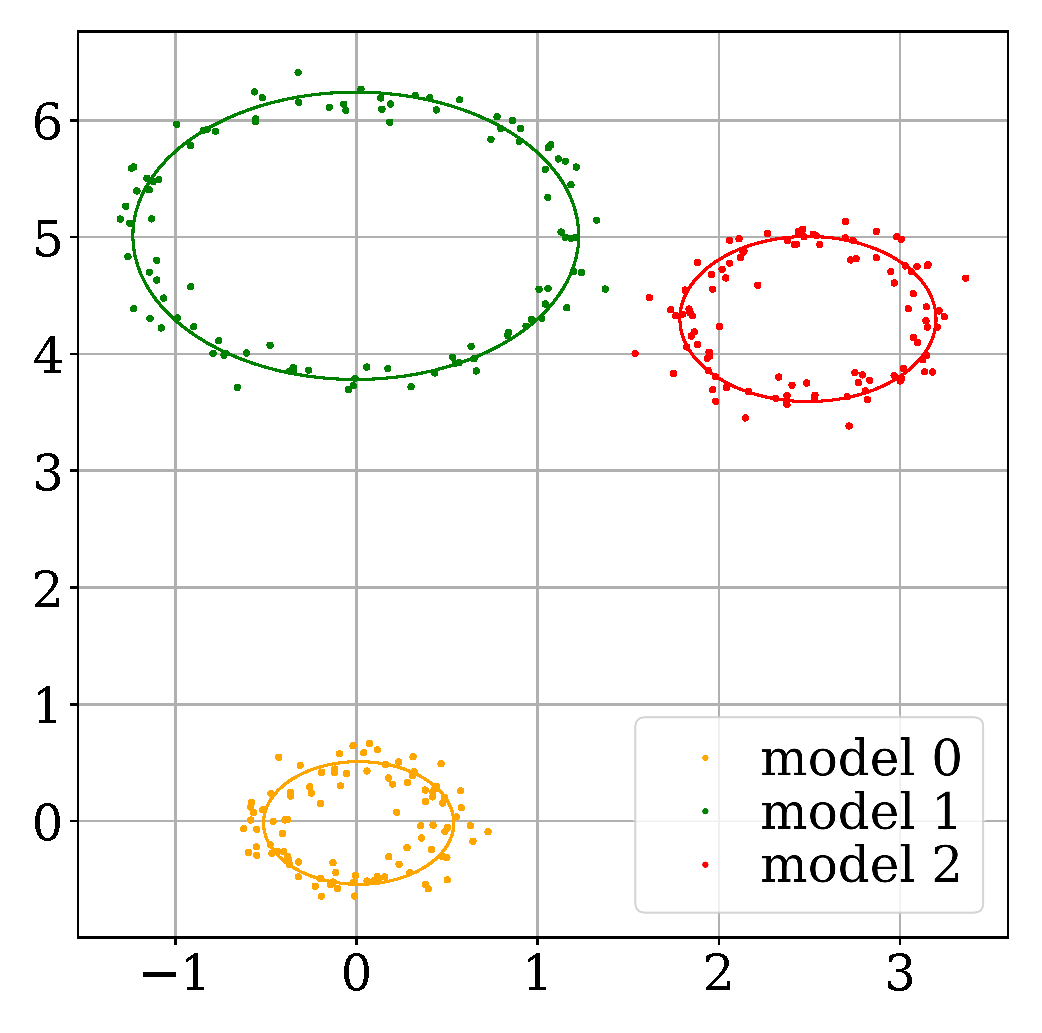
\includegraphics[width =  0.9\textwidth]{figures/901.eps}
\end{minipage}
\begin{minipage}{.25\textwidth}
\vspace{-2.mm}
\hspace{-4.5mm}
      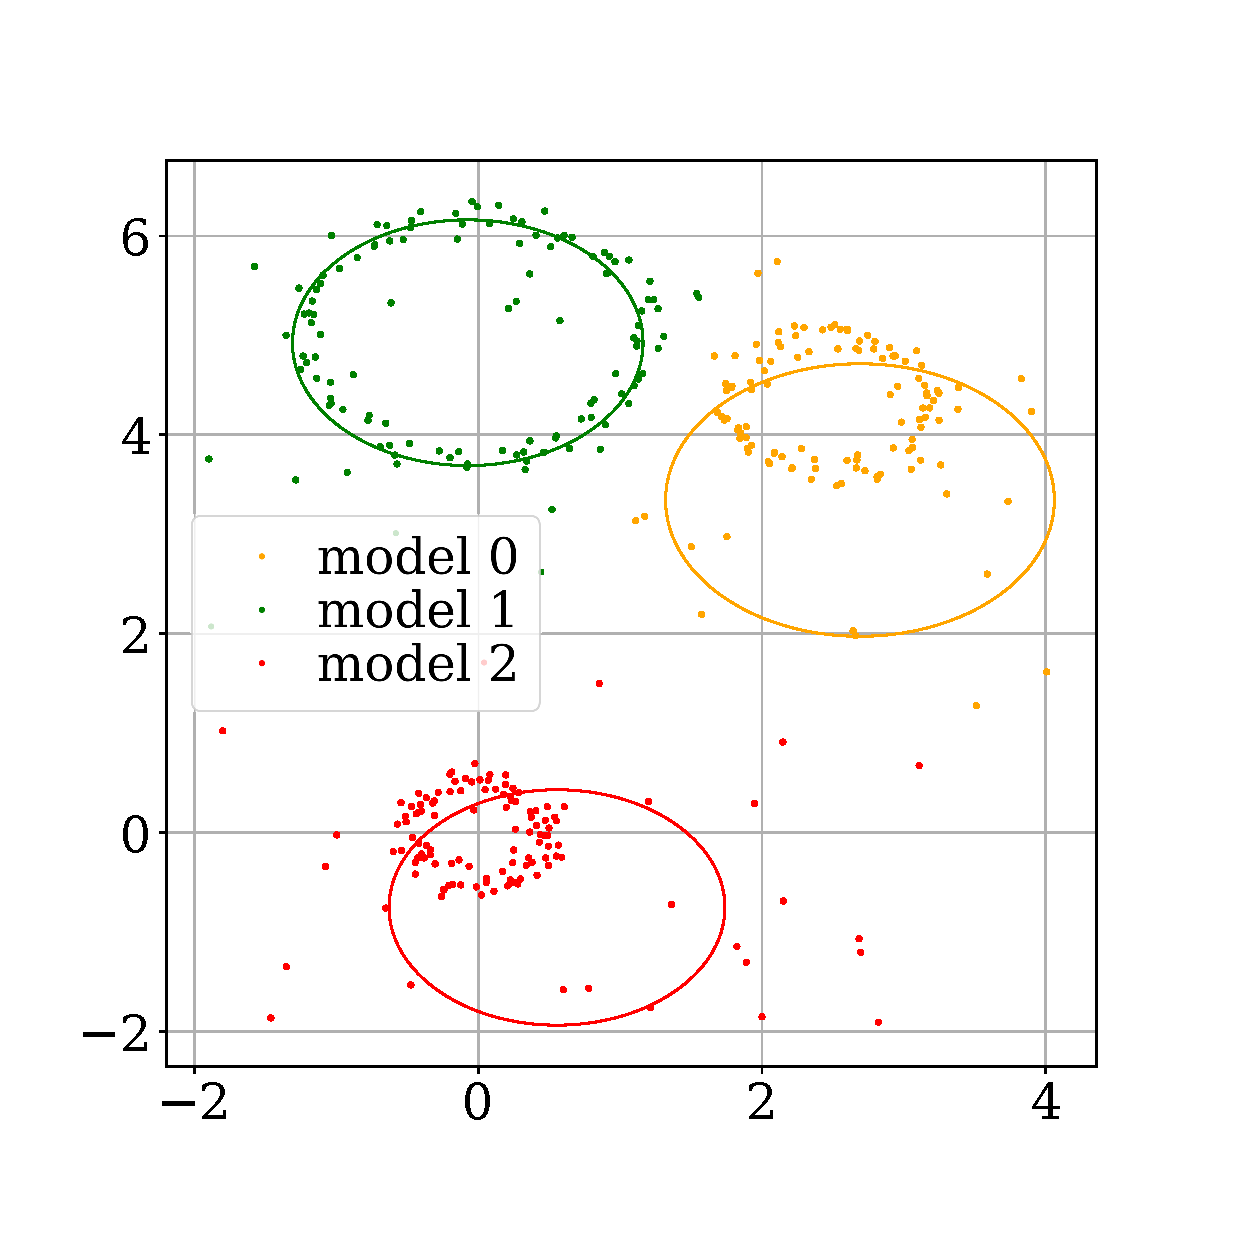
\includegraphics[width =  1.07\textwidth]{figures/902.eps}
\end{minipage}
\begin{minipage}{.25\textwidth}
      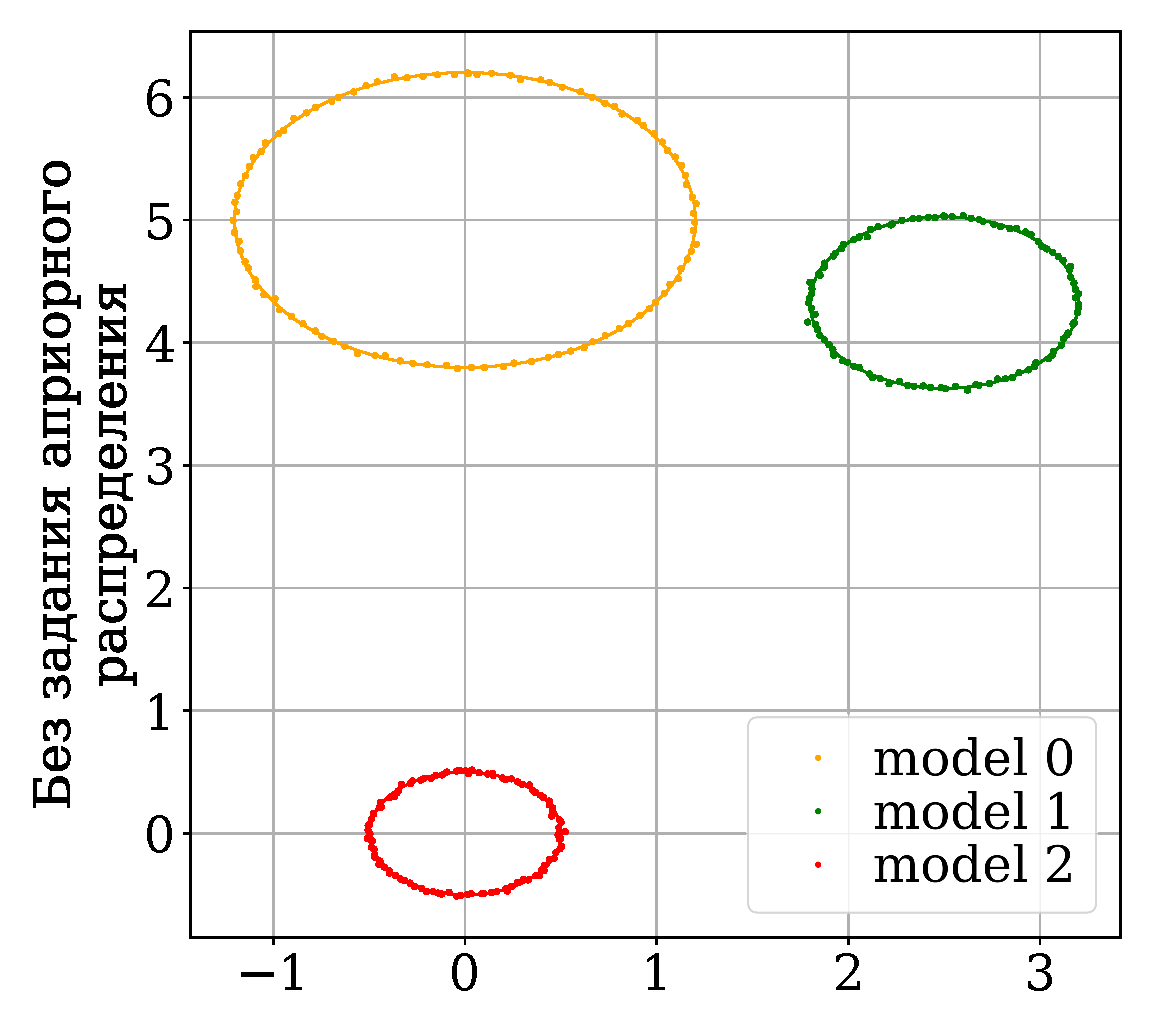
\includegraphics[width =  1.0\textwidth]{figures/900.eps}
\end{minipage}
\begin{minipage}{.25\textwidth}
\hspace{0.3mm}
      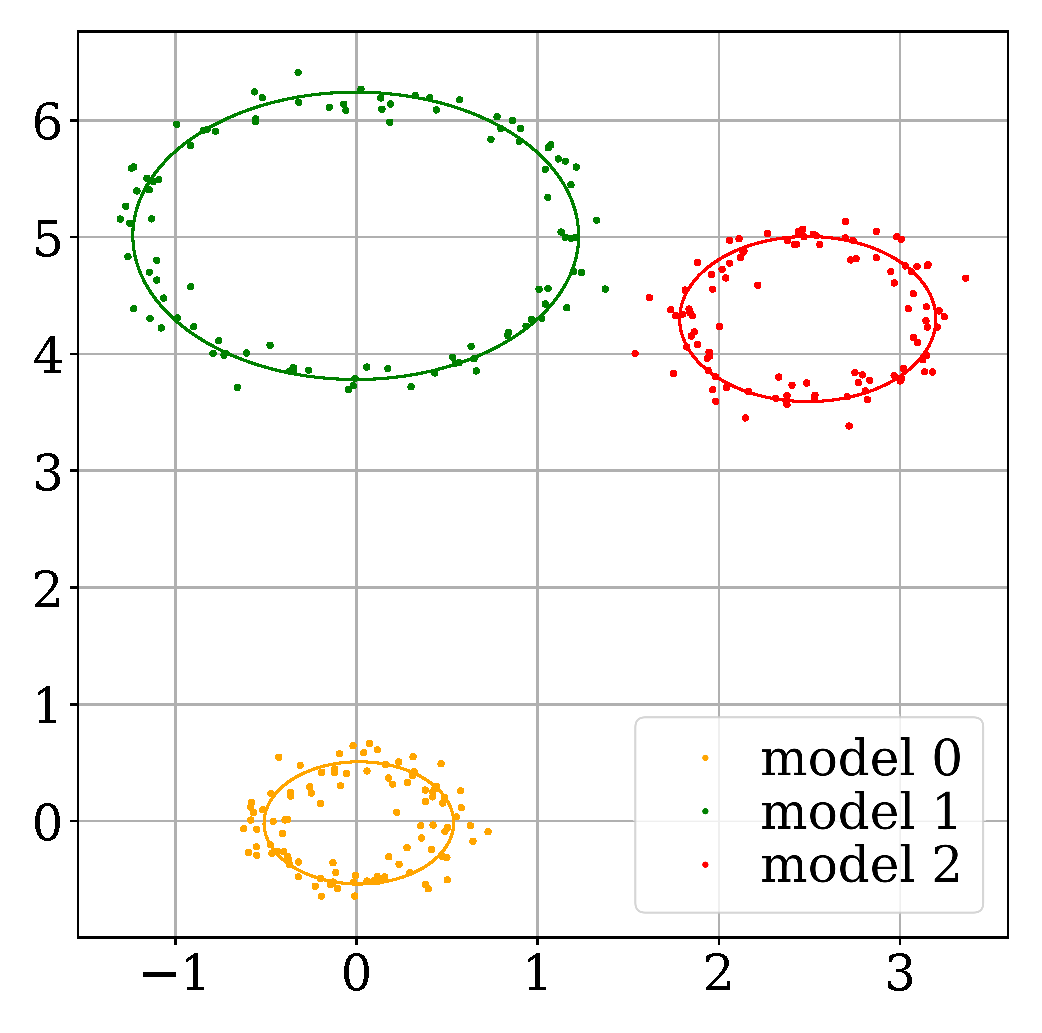
\includegraphics[width =  0.9\textwidth]{figures/911.eps}
\end{minipage}
\begin{minipage}{.25\textwidth}
\hspace{-3.3mm}
      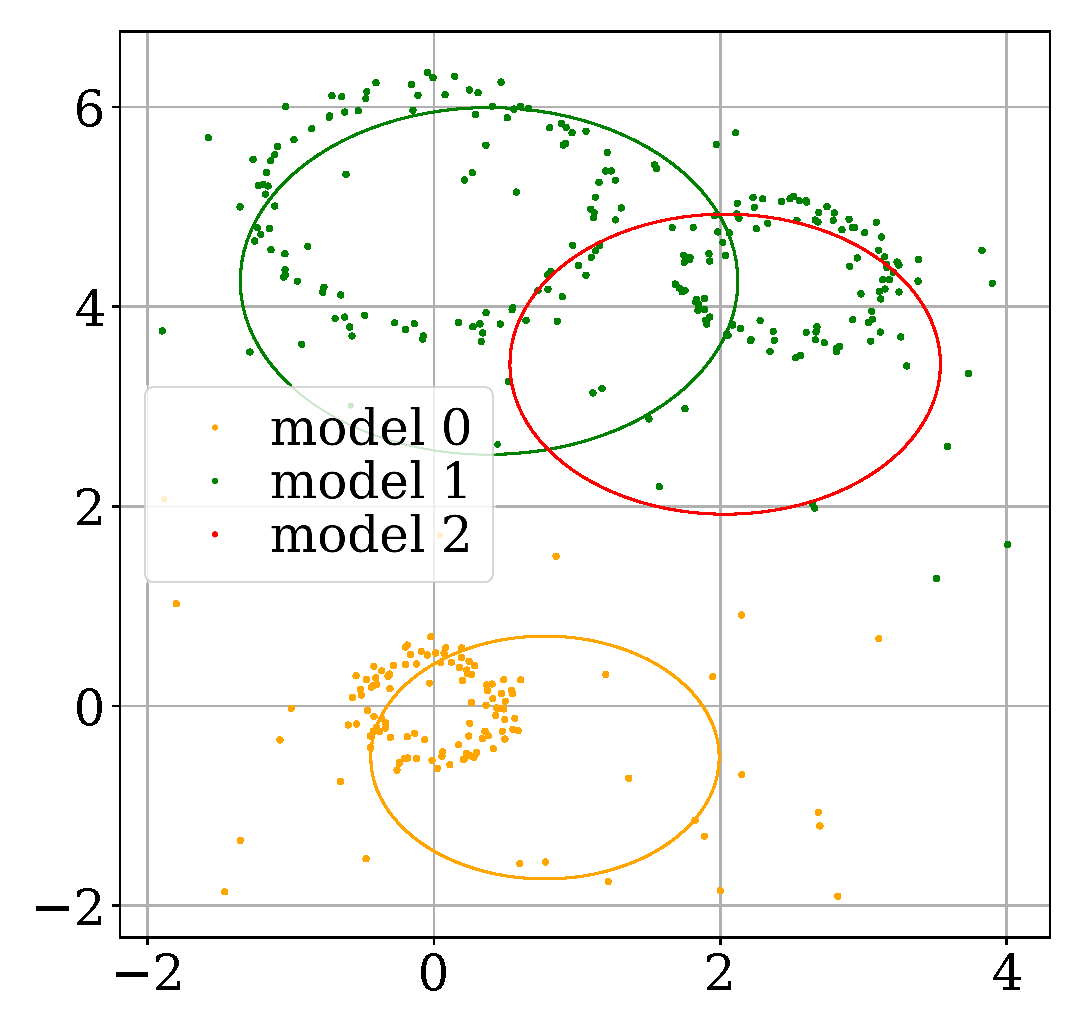
\includegraphics[width =  0.95\textwidth]{figures/912.eps}
\end{minipage}
\end{figure}

\begin{enumerate}
\item Сверху вниз: с заданием априорного распределения; без задания априорного распределения.
\item Слева на право: без шума; шум в радиусе; шум в радиусе окружности и произвольные точки по всему изображению.
\end{enumerate}
При добавлении шума на изображение, качество аппроксимации значительно ухудшается.
\end{frame}
%----------------------------------------------------------------------------------------------------------

\begin{frame}{Эксперимент с разным уровнем шума}
\justifying

\begin{figure}[h]
\begin{minipage}{.27\textwidth}
%\hspace{-3mm}
      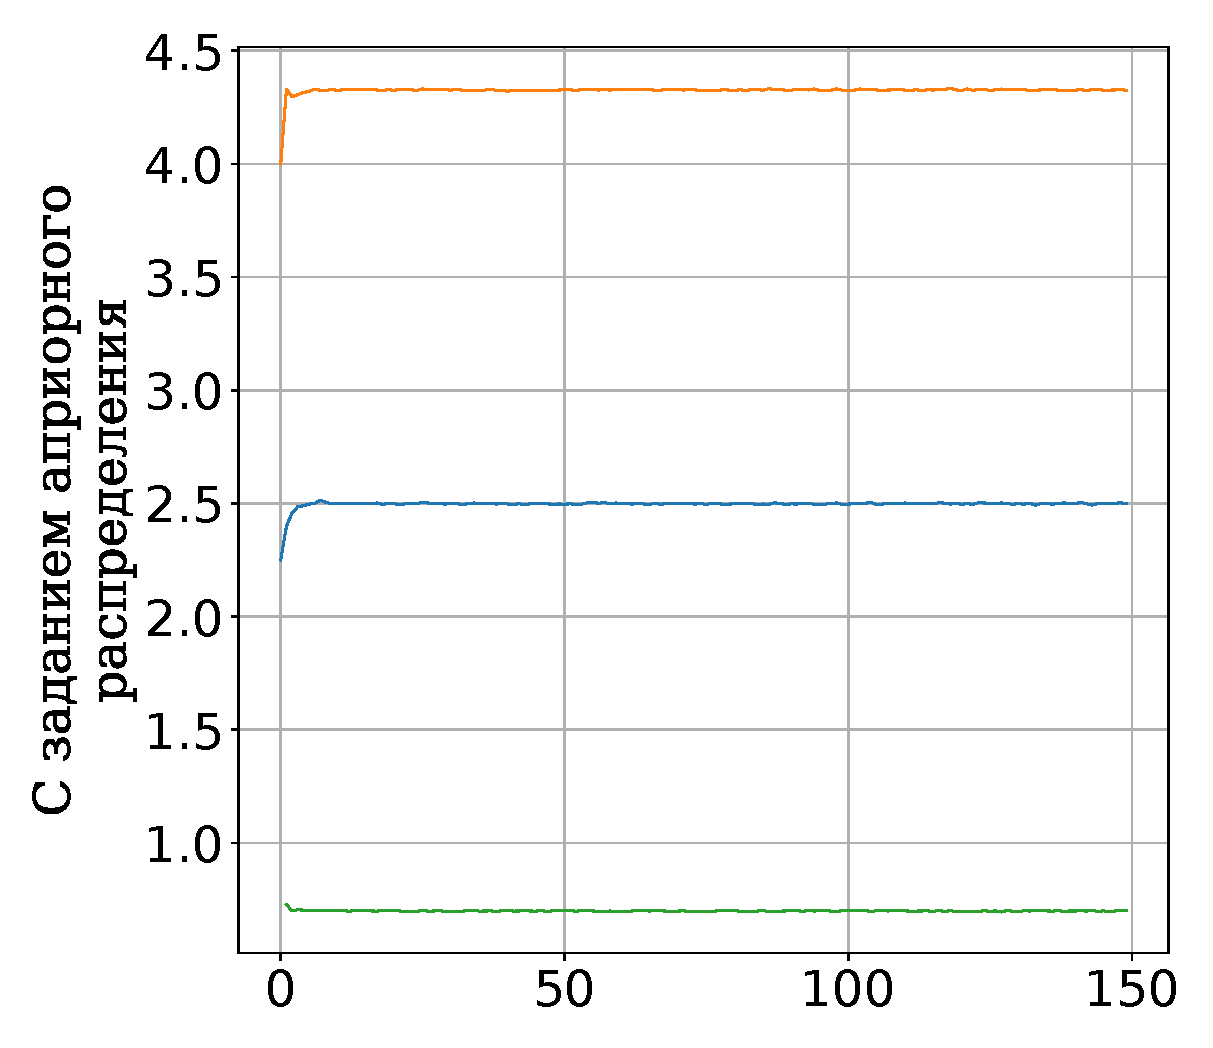
\includegraphics[width = 1.0\textwidth]{figures/910noise.eps}
\end{minipage}
\begin{minipage}{.27\textwidth}
\vspace{0.3mm}
\hspace{1.0mm}
      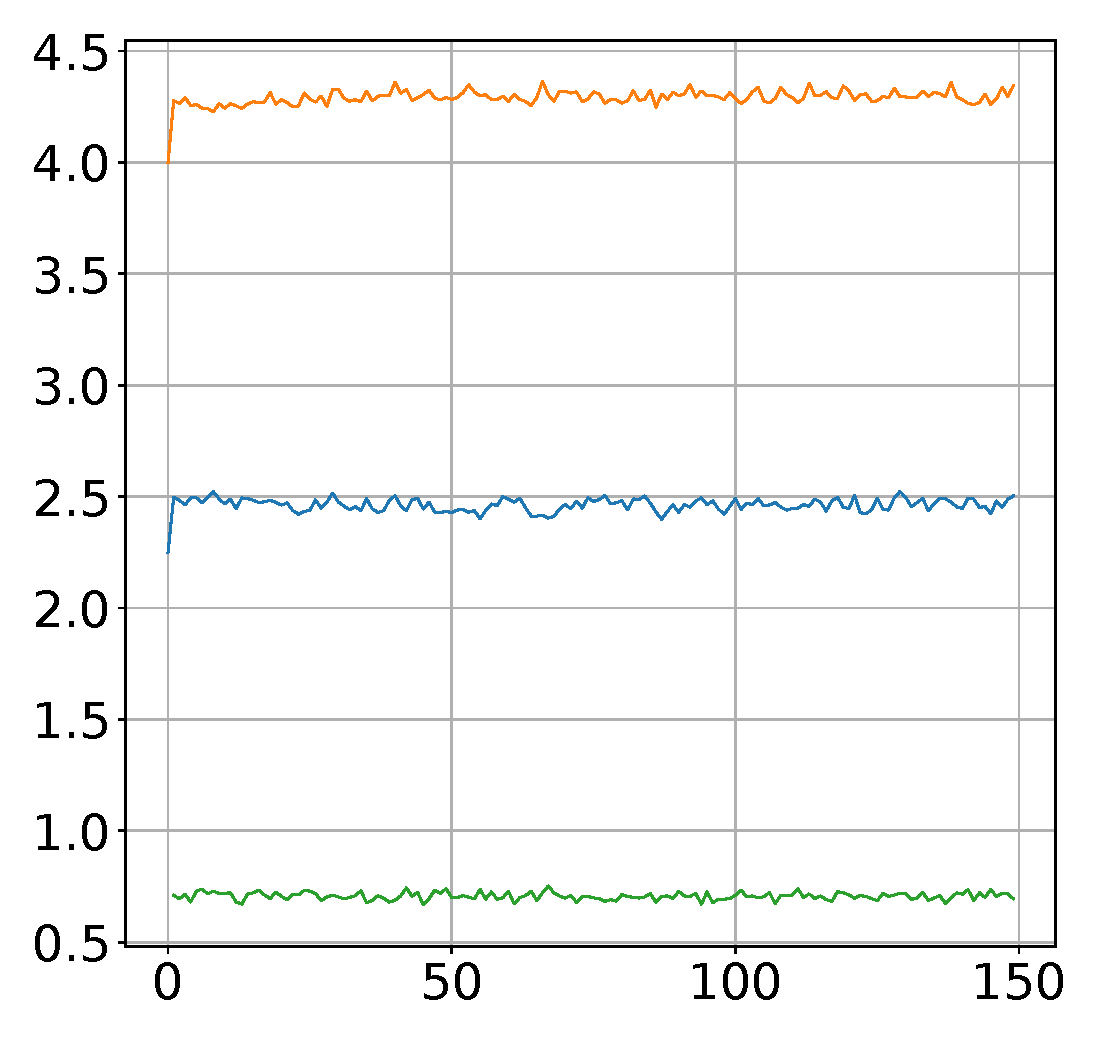
\includegraphics[width = 0.91\textwidth]{figures/911noise.eps}
\end{minipage}
\begin{minipage}{.27\textwidth}
\vspace{0.3mm}
      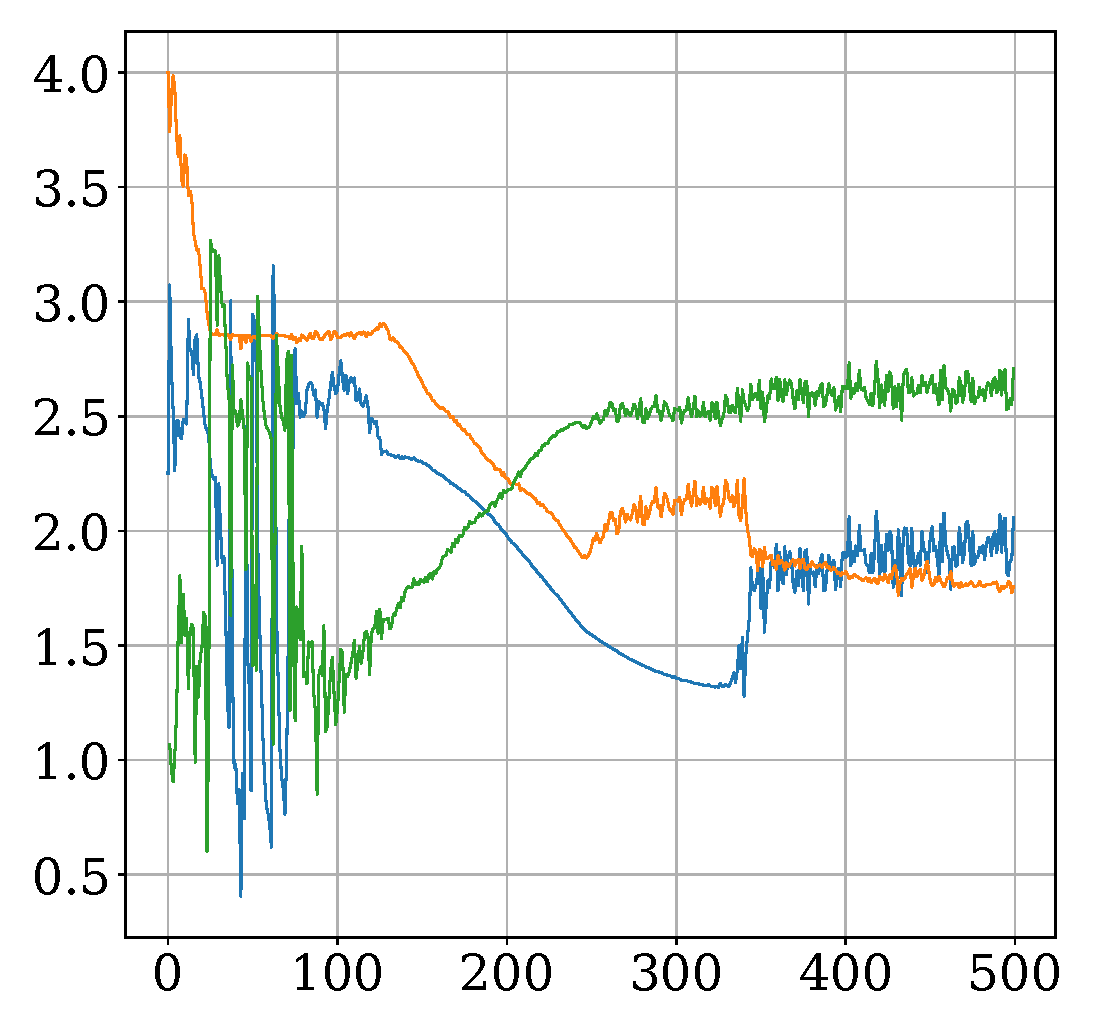
\includegraphics[width = 0.91\textwidth]{figures/912noise.eps}
\end{minipage}
\begin{minipage}{.27\textwidth}
%\hspace{-3mm}
      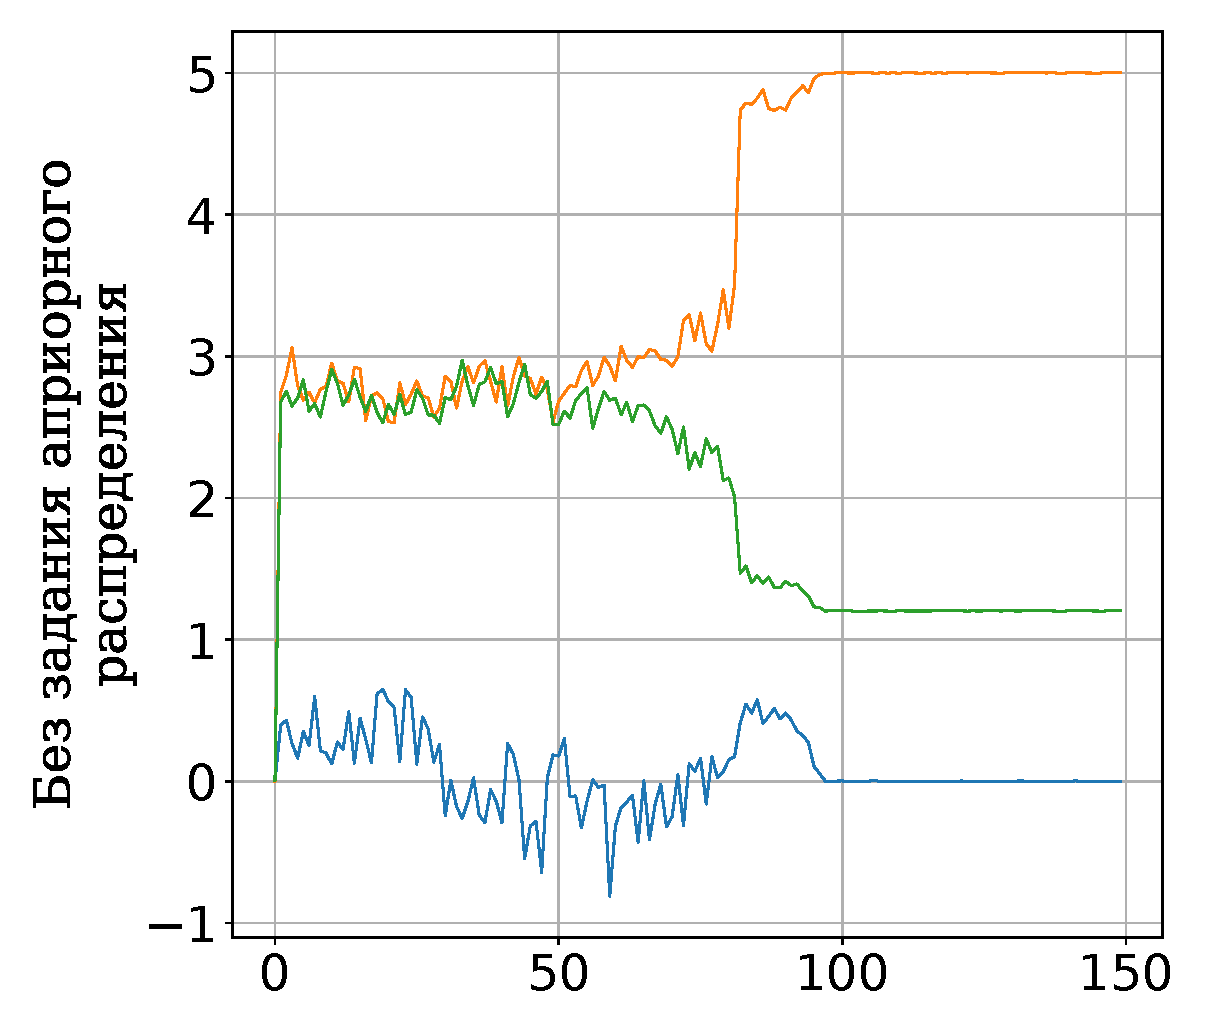
\includegraphics[width = 1.0\textwidth]{figures/900noise.eps}
\end{minipage}
\begin{minipage}{.27\textwidth}
\hspace{-0.4mm}
      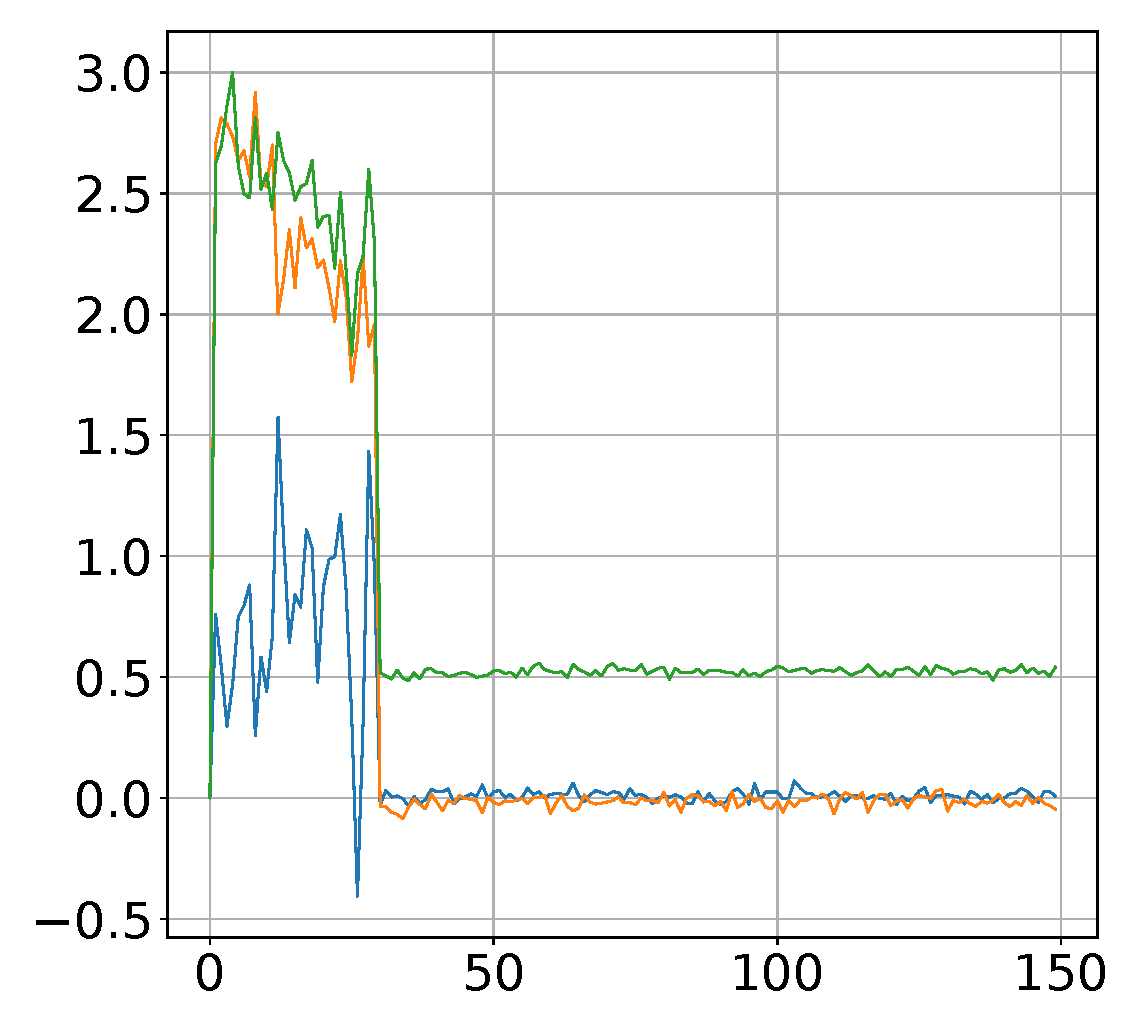
\includegraphics[width = 0.95\textwidth]{figures/901noise.eps}
\end{minipage}
\begin{minipage}{.27\textwidth}
%\hspace{-2mm}
      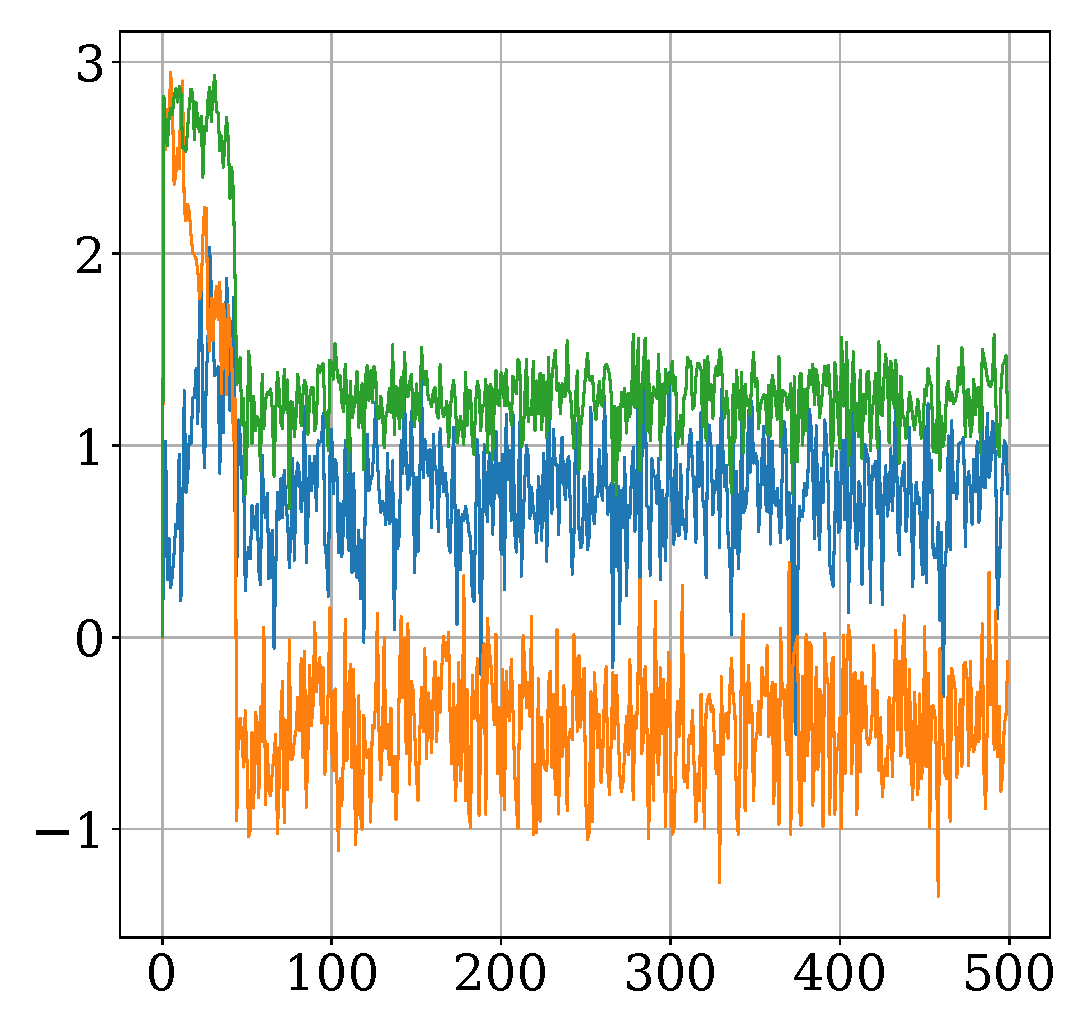
\includegraphics[width = 0.9\textwidth]{figures/902noise.eps}
\end{minipage}
\end{figure}

\begin{enumerate}
\item Сверху вниз: с заданием априорного распределения; без задания априорного распределения.
\item Слева на право: без шума; шум в радиусе; шум в радиусе окружности и произвольные точки по всему изображению.
\end{enumerate}

Модель с заданием априорного распределения является более устойчивой, чем аналогичная без него.

\end{frame}
%----------------------------------------------------------------------------------------------------------

\begin{frame}{Эксперимент с разным уровнем шума}
\justifying

\begin{figure}[h!t]\center
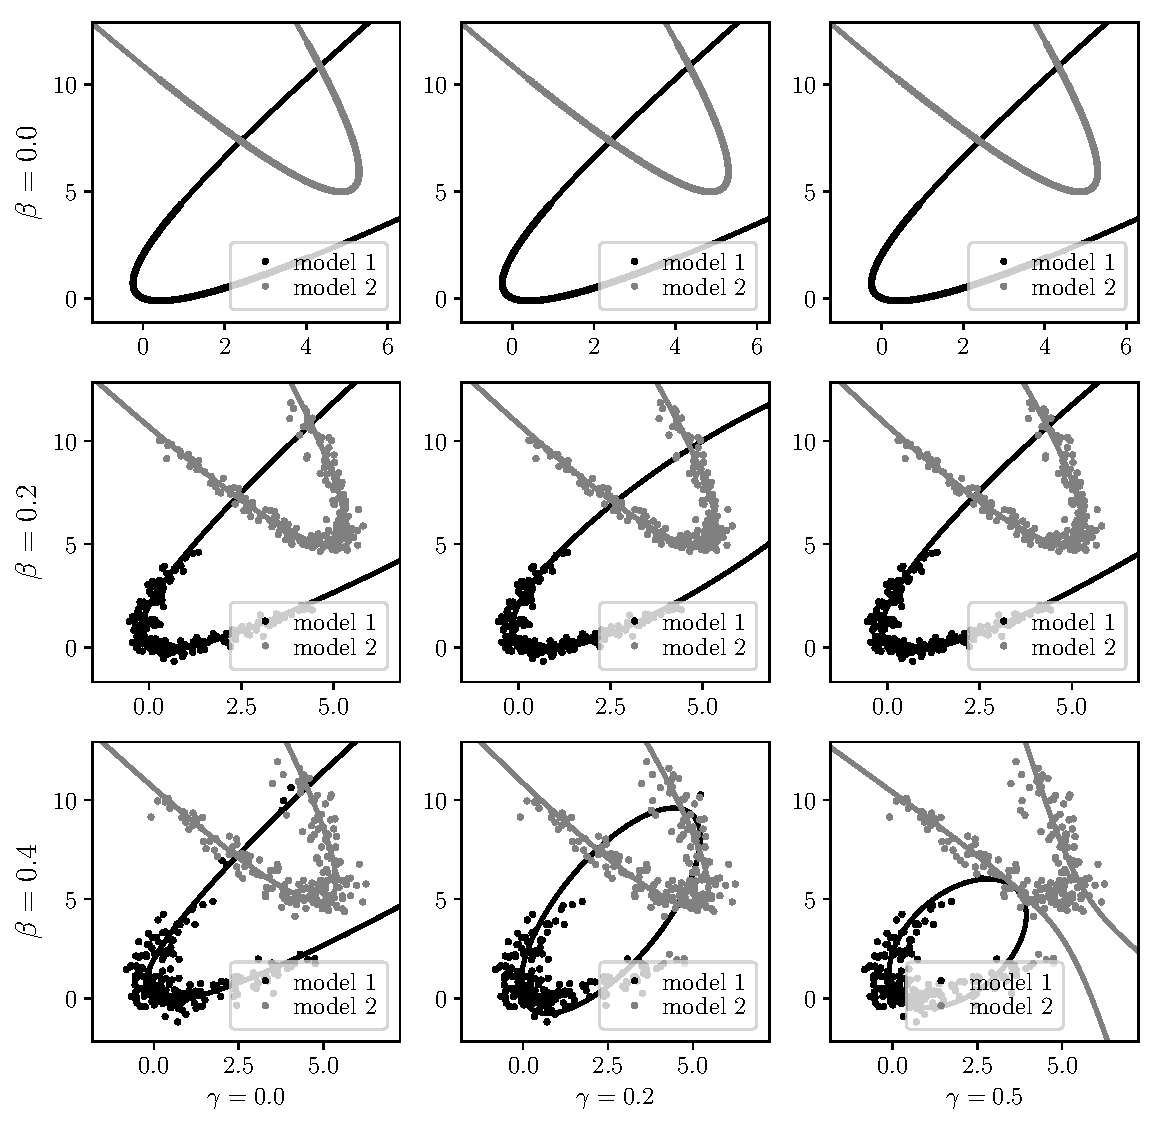
\includegraphics[width=0.6\textwidth]{figures/beta_gamma}
\end{figure}

При малом шуме качество аппроксимации не зависит от параметра~$\gamma$, при увеличении уровня шума, качество аппроксимации зависит от параметра~$\gamma$.

\end{frame}
%----------------------------------------------------------------------------------------------------------

\begin{frame}{Эксперимент с разным уровнем шума}
\justifying

\begin{figure}[h!t]\center
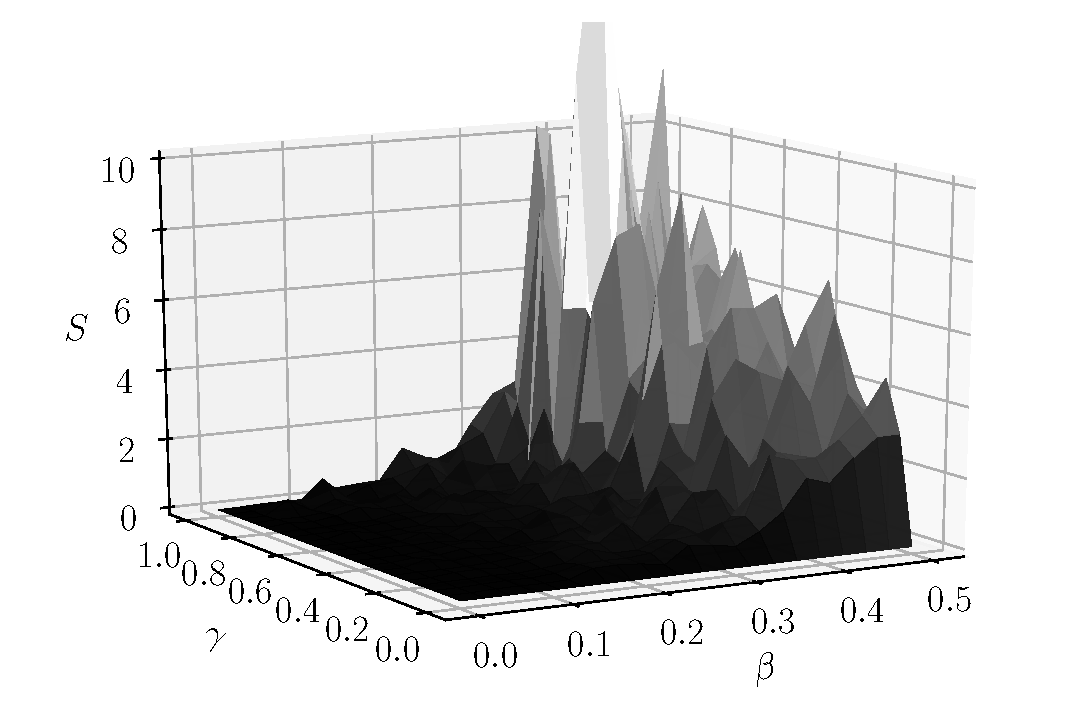
\includegraphics[width=0.8\textwidth]{figures/3dplot}
\end{figure}

При увеличении шума~$\beta$  в данных ошибка аппроксимации~$S$ увеличивается. Параметр~$\gamma$ не сильно влияет при фиксированном параметре~$\beta$.

\end{frame}
%----------------------------------------------------------------------------------------------------------

\begin{frame}{Эксперимент с аппроксимаций радужки глаза}
\justifying

\begin{figure}
     \centering
     \begin{subfigure}[b]{0.3\textwidth}
         \centering
         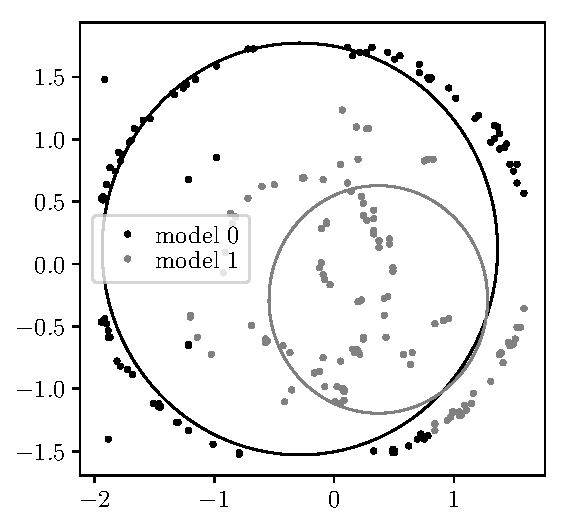
\includegraphics[width=\textwidth]{figures/not_prior_real_example}
         \caption{}
     \end{subfigure}
     \begin{subfigure}[b]{0.3\textwidth}
         \centering
         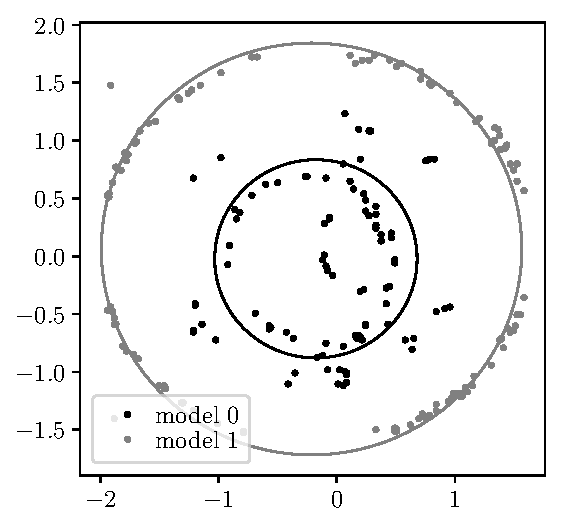
\includegraphics[width=\textwidth]{figures/prior_real_example}
         \caption{}
     \end{subfigure}
     \begin{subfigure}[b]{0.3\textwidth}
         \centering
         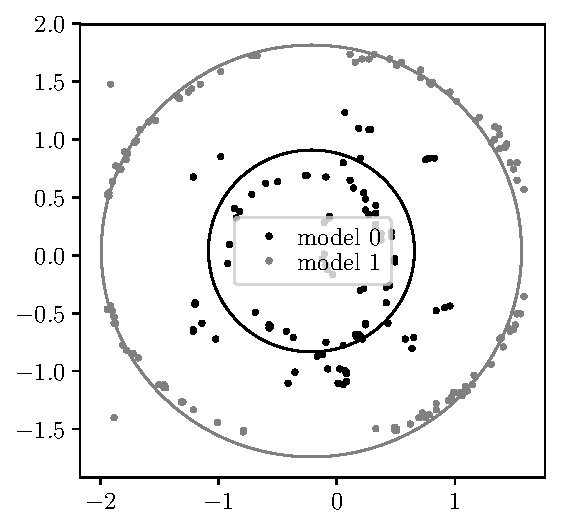
\includegraphics[width=\textwidth]{figures/prior_regular_real_example}
         \caption{}
     \end{subfigure}
\end{figure}

Аппроксимация радужки глаза: a) в случае, если задан регуляризатор $R_0$; b) в случае, если задан регуляризатор $R_1$; b) в случае, если задан регуляризатор $R_2$.

При увеличении сложности регуляризатора с $R_0$ до $R_2$ качество аппроксимации улучшается.

\end{frame}
%----------------------------------------------------------------------------------------------------------

\begin{frame}{Визуализация сходимости}
\justifying
Регуляризация априорных распределений
\begin{center}
	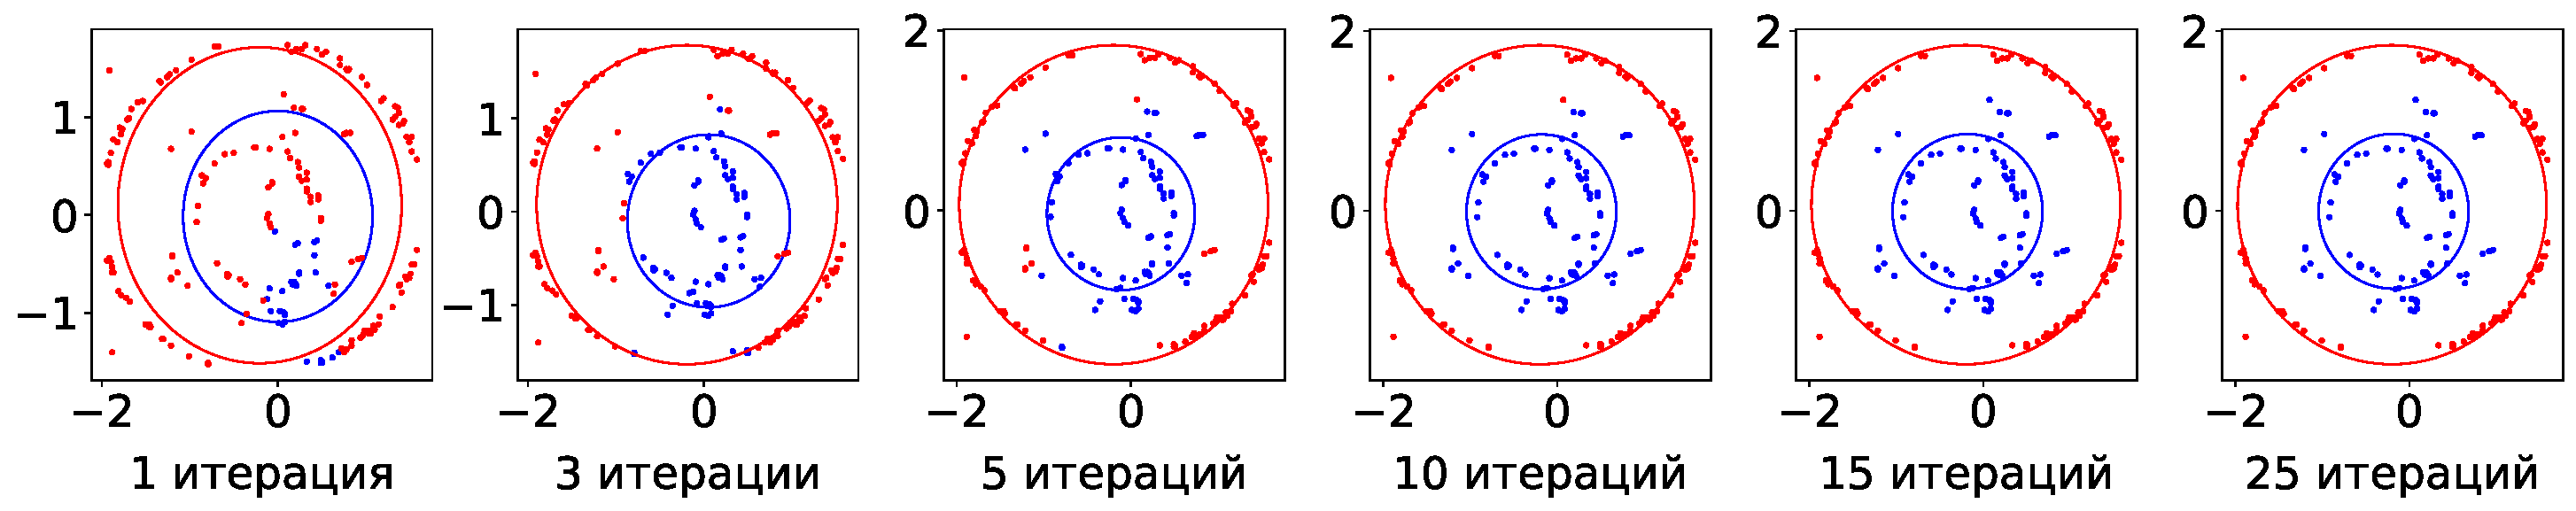
\includegraphics[width=0.85\textwidth]{figures/experiment_real_regular}
\end{center}
С заданием априорного распределения на модели
\begin{center}
	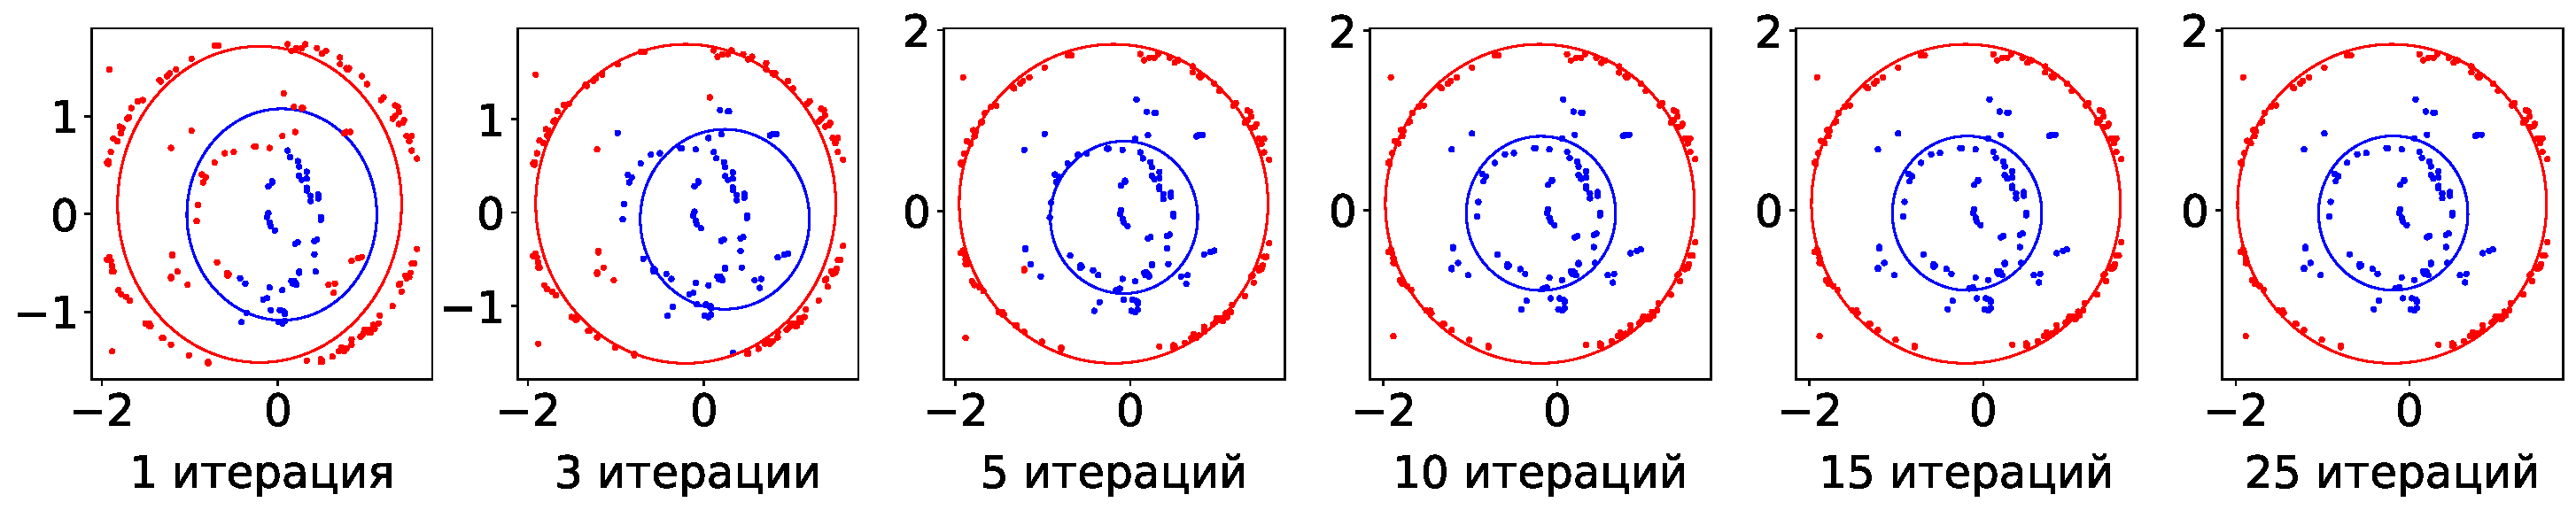
\includegraphics[width=0.85\textwidth]{figures/experiment_real_prior}
\end{center}
Без задания априорного распределения
\begin{center}
	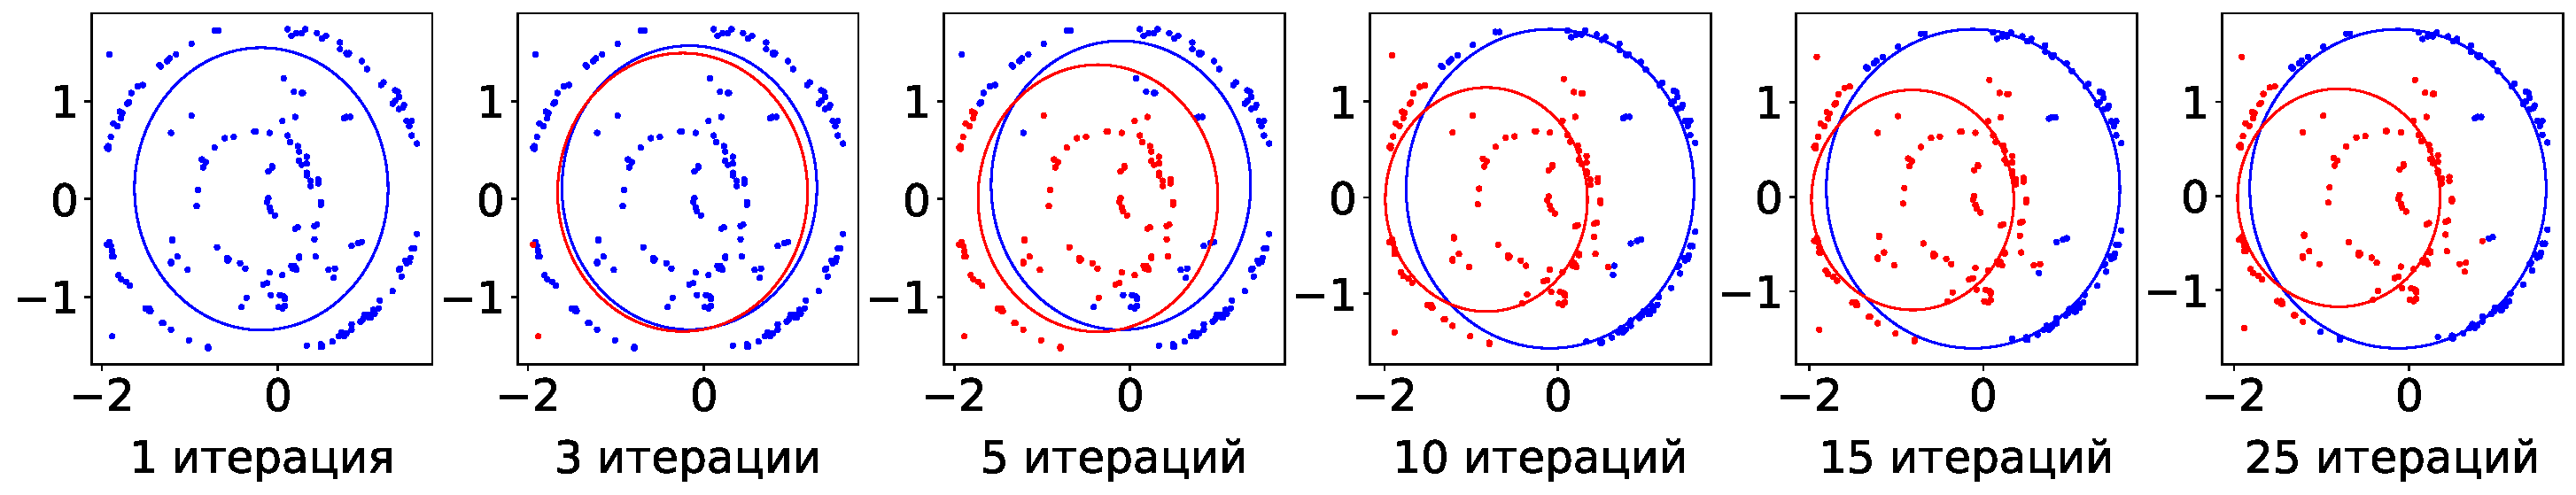
\includegraphics[width=0.85\textwidth]{figures/experiment_real_not_prior}
\end{center}
\end{frame}
%----------------------------------------------------------------------------------------------------------

\begin{frame}{Заключение}
\justifying
	\begin{enumerate}
	\justifying
		\item Поставлена задача обучения с экспертной информацией.
		\item Предложен метод решения задачи обучения с экспертной информацией.
		\item Приведен частный случай обучения с экспертной информацией для решения задачи поиска кривых второго порядка.
		\item Введено понятие регуляризации априорных распределений для улучшения качества мультимодели.
		\item Проведен вычислительный эксперимент для анализа предложенной модели.
	\end{enumerate}

~\\

Планируется:
	\begin{enumerate}
	\justifying
		\item Улучшить мультимодель при помощи задания априорного распределения на шлюзовую функцию.
		\item Рассмотреть в качестве локальных моделей не только модели, которые описывают данные, а также модель, которая отвечает за шум в данных.
		\item Провести адаптация предложенного метода для методов глубокого обучения.
	\end{enumerate}	

\end{frame}
%----------------------------------------------------------------------------------------------------------

\begin{frame}{Публикации ВАК по теме}
\justifying
\begin{enumerate}
\item \textit{Грабовой\;А.\,В., Бахтеев\;О.\,Ю., Стрижов\;В.\,В.} Определение релевантности параметров нейросети // Информатика и ее применения, 2019, 13(2).
\item \textit{Грабовой\;А.\,В., Бахтеев\;О.\,Ю., Стрижов\;В.\,В.} Введение отношения порядка на множестве параметров аппроксимирующих моделей // Информатика и ее применения, 2020, 14(2).
\item \textit{A.\;Grabovoy, V.\;Strijov.} Quasi-periodic time series clustering for human. Lobachevskii Journal of Mathematics, 2020, 41(3).
\item \textit{Грабовой\;А.\,В., Стрижов\;В.\,В.} Анализ выбора априорного распределения для смеси экспертов // Журнал Вычислительной математики и математической физики, 2021. 61(5).
\item \textit{Грабовой\;А.\,В., Стрижов\;В.\,В.} Анализ моделей привилегированного обучения и дистилляции // Автоматика и телемеханика, 2021 (текущая работа, на рецензировании).
\item \textit{T.\;Gadaev, A.\;Grabovoy, A.\;Motrenko, V.\;Strijov} Numerical methods of minimum sufficient sample size estimation for linear models // in progress.
\item \textit{Базарова\;А.\,И., Грабовой\;А.\,В., Стрижов\;В.\,В.} Анализ свойств вероятностных моделей в задачах обучения с экспертом // подано.
\end{enumerate}

\end{frame}
%----------------------------------------------------------------------------------------------------------

\end{document} 